\documentclass{article}
\usepackage[utf8]{inputenc}
\usepackage{graphicx}
\usepackage{float}
\usepackage{hyperref}

\usepackage{etoolbox} %required for cover page
\usepackage{booktabs}
\usepackage[usestackEOL]{stackengine}
\usepackage[T1]{fontenc}
\usepackage[utf8]{inputenc}
\usepackage{bm}
\usepackage{graphicx}
\usepackage{subcaption}
\usepackage{amsmath}
\usepackage{amsfonts}
\usepackage{mathtools}
\usepackage{xcolor}
\usepackage{float}
\usepackage{hyperref}
\usepackage[capitalise]{cleveref}
\usepackage{enumitem,kantlipsum}
\usepackage{amssymb}
\usepackage[square,numbers,sort]{natbib}
\usepackage[ruled,vlined]{algorithm2e}
\usepackage{listings}
\usepackage{minted}
\usemintedstyle{emacs}

\begin{document}

\begin{flushright}
   \rule{14cm}{5pt}\vskip1cm
    \begin{bfseries}
        \Huge{PARALLEL ALGORITHMS FOR EVALUATING MATRIX POLYNOMIALS }\\
        \vspace{1.5cm}
        \LARGE{Under the guidance of : Dr. Chandresh Kumar}\\
        \vspace{1.5cm}
         IIT Indore Computer Science and Engineering\\
        \vspace{1.5cm}
         Purnadip Chakrabarti      - 190002048\\
         Garvit Galgat         - 190001016\\
         Vaibhav Chandra       - 190001065\\
         Peddamallu Bhuvana Sree - 190001046\\
         \vspace{1.5cm}
    \end{bfseries}
\end{flushright}


\section{Abstract}
In this paper, we put forward a technique to efficiently evaluate matrix polynomials. There are several building blocks in this technique. Each of them perform a designated task. We also parallelize this technique to further improve the runtime of the algorithm. We see that the algorithm based on applying Paterson-Stockmeyer algorithm to entire matrix proves to be slow for large input matrices but is easily parallelizable. Another algorithm based on Schur Decomposition is then proposed and integrated to make a hybrid algorithm.


\section{Introduction}
Given a real or complex matrix A and a polynomial q with coefficients $c_0,c_1,..c_d$, we wish to compute the following matrix 
\begin{figure}[H]
 \includegraphics[]{ps.png}
\end{figure}
Naive algorithm to solve this problem performs about d-1 matrix multiplications. The overall time complexity for such an algorithm is $\Theta(n^{\omega}d)$, where $\Theta(n^{\omega})$ is the complexity for matrix multiplication $\omega$ is 3 for conventional matrix multiplication and $\omega$ $\approx$ 2.7 for strassen based matrix multiplication. \par
An important way of looking at this problem is by rearranging the polynomial, done by the Paterson and Stockmeyer algorithm. q(A) is rearranged so that it is converted into a polynomial in a power p for p < d with coefficients themselves being polynomials of degree at most p - 1. Complexity of the algorithm depends on the choice of p. A good p leads to a complexity of $\Theta(n^{\omega}\sqrt{d})$ Our technique uses this algorithm either on A itself or schur decomposition of A that we see later. \par
Another important idea is the parlett's algorithm that reduces the matrix A to its Schur form A = QTQ*, evaluates the function for the diagonal elements of T and then uses recurrence equation to compute for the off-diagonal elements and then finally multiplies back Q to form q(A) = $Qq(T)Q^*$. The complexity of this technique is $\Theta(n^{3})$. Unfortunately, parlett's algorithm is numerically unstable. A variant of the same by Davies and Higham fixes this issue by reordering the eigenvalues to make contiguous clusters of nearly equal eigenvalues. We abstain from using this approach in our algorithm due to its very complicated implementation and less room for parallelization. We continue with parlett's algorithm in this paper.  
Asymptotically, the parlett algorithm is always preferable but the constants involved in Schur decomposition is high. So in practise, its only beneficial to use parlett's algorithm when the d is large otherwise the Paterson-Stockmeyer gives better result. All this leads to the following flow of our algorithm.

\begin{figure}[H]
 \centering
 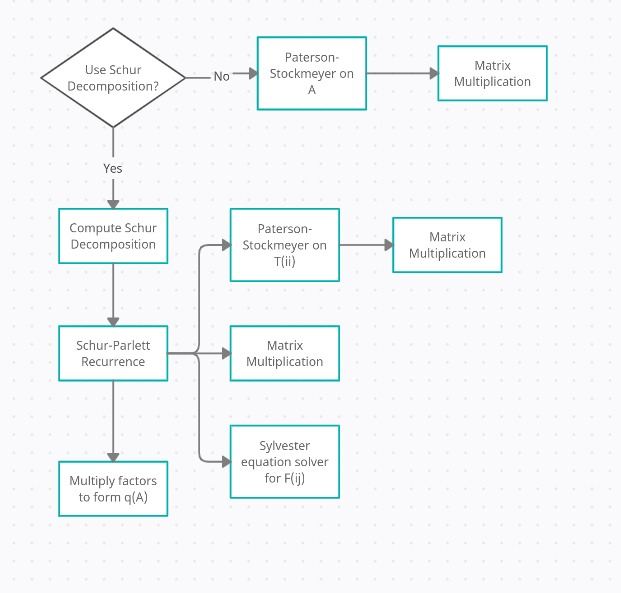
\includegraphics[width=12cm]{flowchart.jpeg}
\end{figure}

We also try and parallelize each individual component of the algorithm. Some are easy and straightforward (matrix multiplication) but some are rather tricky (Schur decomposition). We parallelize the components we can otherwise we improve it as much as we can. 



\section{Algorithmic Design}

Our algorithm considers two approaches. If the input matrix A is sufficiently small then it does not do the expensive Schur decomposition and applies Paterson-Stockmeyer directly to A instead. The complexity of this approach is $\Theta(n^{\omega}\sqrt{d})$ along with parallelism. \par
If dimensions of A is rather large and the degree of polynomial is high then our algorithm computes the Schur decomposition, where Q is unitary and T is upper triangular. If A is real but has complex eigenvalues then T is block triangular with blocks of size 1-by-1 or 2-by-2. Now the task reduces to evaluating q(T). T, being upper triangular, reduces the cost of computing q drastically. After we obtain q(T), we can calculate q(A) = $Qq(T)Q^*$ using just two matrix multiplications. \par
We calculate q(T) using parlett's algorithm. First of all, $t_i_i$ is calculated for all diagonal elements. The cost of this step is $\Theta(nd)$. Then we use the recurrence relation to compute ij element of q(T). The cost of this step is $\Theta(n^3d)$. We avoid the case involving A having equal eigenvalues due to the unstable nature of parlett's recurrence. \par


\subsection{Paterson-Stockmeyer Polynomial Evaluation}\par
The paterson-stockmeyer method expresses q(A) as
\begin{figure}[H]
 \centering
 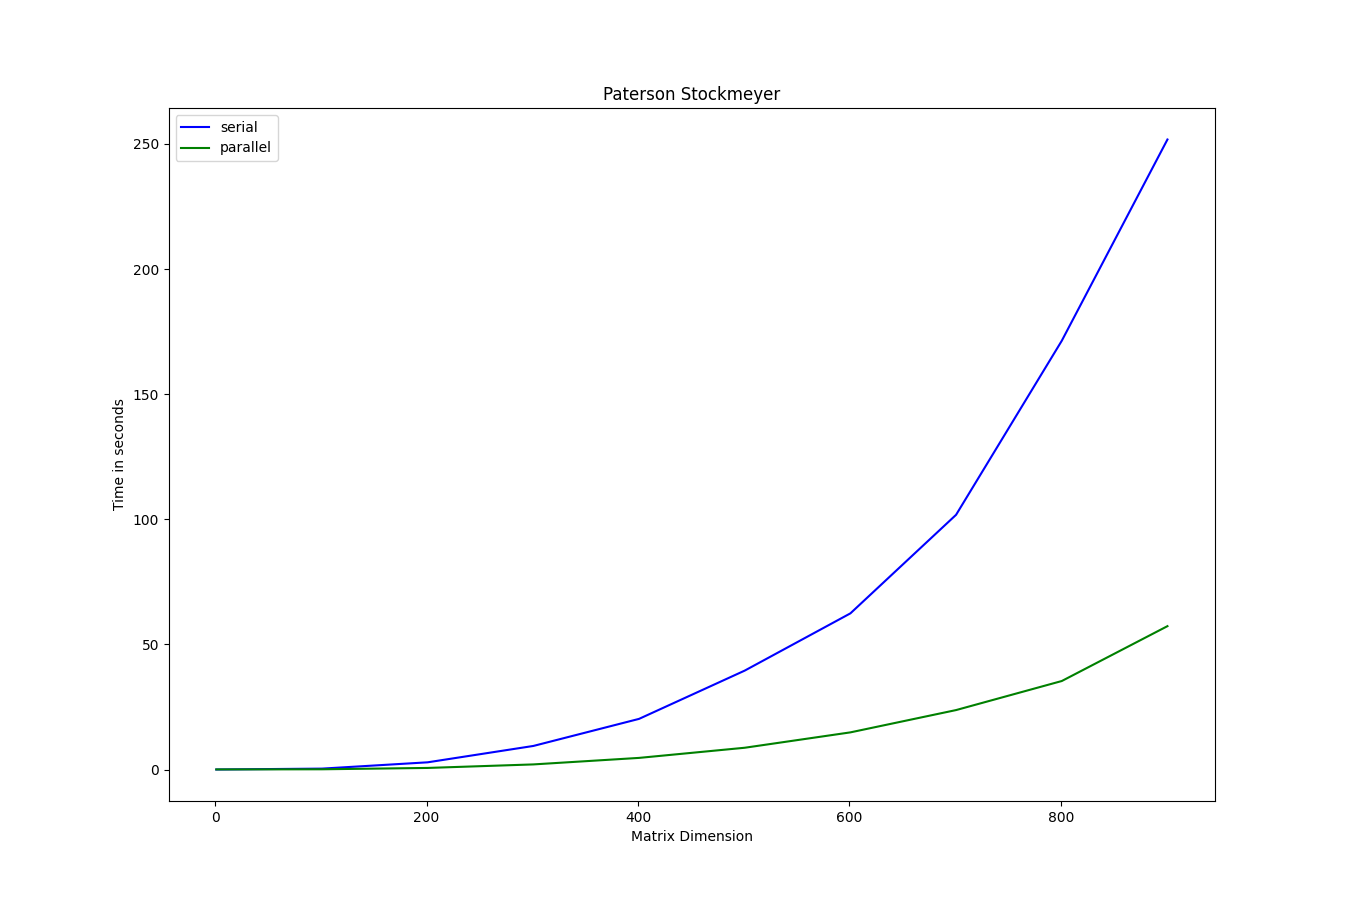
\includegraphics[]{paterson.png}
\end{figure}
where p and s are integers such that ps > d. The best arithmetic efficiency is obtained when p $\approx$ s $\approx$ $\sqrt{d}$. The algorithm first evaluates and stores $A^{2},...,A^{p-1},A^{p}$. These steps can be carried out sequentially in $\Theta(\sqrt{d})$ matrix multiplication steps (each highly parallelizable).\par
Once $I,A,A^{2},...,A^{p-1}$ are stored, we can evaluate all the coefficient polynomials
\begin{figure}[H]
 \centering
 \includegraphics[]{coefficient_poly.png}
\end{figure}
We have used Horners's rule on $A^{p}$ to evaluate coefficient polynomials. In each step we multiply the accumulator in which we build up q(A) by $A^{p}$ and add the next coefficient polynomial to the accumulator. The critical path is $\Theta(slog(n)) \approx \Theta(\sqrt{d}log(n))$.

\subsection{Schur Decomposition}

We know that having a triangular matrix as an input reduces the runtime significantly. The best method convert a matrix into its diagonal form is by Schur Decomposition. The Schur Decomposition factors A into A = $QTQ^H$ where Q is a unitary matrix and T is an upper triangular matrix. The eigenvalues of A are present on the diagonals of T. \par
If A is real with complex eigenvalues then T is complex too. Real Schur form of a A will a quasi-upper triangular matrix with 1-by-1 and 2-by-2 blocks where each 2-by-2 block is standardized in the form [a b/ c d] b.c < 0 . Eigenvalues of such a block is a $\pm$ i$\sqrt{bc}$ \par
The most convenient way of calculating Schur form is by the QR algorithm. f(A) = $Qf(T)Q^H$ , therefore, our task reduces to calculating f for an upper triangular matrix T. Consequently, here on our focus will be on solving f for upper triangular matrix.

\subsection{Sylvester Equation Solver}
In parlett recurrence the off-diagonal blocks $F_i_j$ are defined as the solution of a Sylvester equation.
\begin{figure}[H]
 \centering
 \includegraphics[]{sylvester_eq.png}
\end{figure}
Hence, this algorithm is used to solve off-diagonal blocks.We know a sylvester equation of form $AX - XB = C$ can be written as $mx = c$, where $m = (I * A - B^t * I)$ (here * is kronecker product) and x, c are obtained by stacking all columns of X and C from right to left. We can solve the equation $mx = c\quad  =>\quad  x = m^(-1)c$\quad  using gauss elimination. X can be obtained by restacking columns of x. We have solved the equation(4) using above steps.


\subsection{Parlett Recurrence}
Parlett Recurrence is an elegant way of calculating f for an upper triangular matrix. We start by calculating f for each diagonal block ( we will use paterson-stockmeyer algorithm for this). To calculate F(ij) we will then employ the following recurrence in a bottom-top left-right fashion. 

Due to the denominator term, parlett recurrence breaks down incase of repeated eigenvalues or even for eigenvalues that are very close to each other. A blocked parlett recurrence can be used to handle the case for repeated eigenvalues.

\section{Implementation and Parallelization}

\subsection{Schur Decomposition}




\subsection{Sylvester Equation Solver}



\subsection{Parlett Recurrence}

\section{Evaluation}

\section{Conclusion}



\end{document}